\documentclass[12pt]{article}
\usepackage{ctex}
\usepackage[english]{babel}
\usepackage{blindtext}
\usepackage{nameref}
\usepackage{fancyhdr}
\usepackage{amsmath,amssymb,amsthm}
\usepackage{graphicx,float}
\usepackage{physics}
\usepackage{pgfplots}
\usepackage[a4paper, total={6in, 9in}]{geometry}

\graphicspath{{../image/}}

\pagestyle{fancy}
\fancyhf{}
\fancyhf[HL]{二項式定理}
\fancyhf[CF]{\thepage}

\newcommand{\innerprod}[2]{\langle{#1},{#2}\rangle}
\newcommand{\id}{\mathtt{id}}

\newtheorem{definition}{定義}
\newtheorem*{theorem}{定理}
\newtheorem*{corollary}{衍理}
\newtheorem*{lemma}{引理}
\newtheorem*{proposition}{設理}
\newtheorem*{remark}{小記}
\newtheorem*{claim}{主張}
\newtheorem*{example}{例子}
\newtheorem*{axiom}{公設}
\renewenvironment*{proof}{\textit{證明.}}{\hfill$\qed$}

\newenvironment*{sol}{\par \textbf{解}.}{\hfill$\blacksquare$}

\begin{document}
    \section*{階乘}

    階乘為一種特別的乘積,定義如下:

    \begin{definition}[階乘]
        對任意正整數$n$,定義$$n!=\prod_{i=1}^n i=1\cdot2\cdot3\cdot\cdots\cdot (n-1)\cdot n$$

        並定義$0!=1$.
    \end{definition}

    \begin{example}
        $1!=1$.
    \end{example}

    \begin{example}
        $2!=2\cdot 1!=2$.
    \end{example}

    \begin{example}
        $3!=3\cdot 2!=6$.
    \end{example}

    \begin{example}
        $4!=4\cdot 3!=24$.
    \end{example}

    \begin{example}
        對於$0!$的定義,可以如此理解:$n!=n(n-1)!$,則$(n-1)!=\frac{n!}{n}$。因此,$$0!=(1-1)!=\frac{1!}{1}=1$$
    \end{example}

    \begin{remark}
        階乘的運用只限非負整數;若需要對階乘進行拓展,可參考伽馬函數:$$\Gamma(s):=\int_0^\infty t^{s-1}e^{-t}dt$$
    \end{remark}

    \section*{組合}

    \begin{definition}[組合數]
        對於從$n$項物品中隨機抽取$r$項物品的組合數,定義爲$$C_r^n=\frac{n!}{r!(n-r)!}.$$
    \end{definition}

    \begin{example}[HKDSE MA 2019 I-15]
        設一班有21男與11女,若從班裏抽取5人成爲班會成員,並有至少1男,則有多少種不同的班會組合?
        \begin{sol}
            至少有1男,則全部組合方式排除沒有男生的組合方式:\begin{align*}
                C_5^{21+11}-C_5^{11}=200914
            \end{align*}
        \end{sol}
    \end{example}

    \begin{example}
        數出下圖中純長方形與正方形的數量。
        \begin{figure}[H]
            \centering
            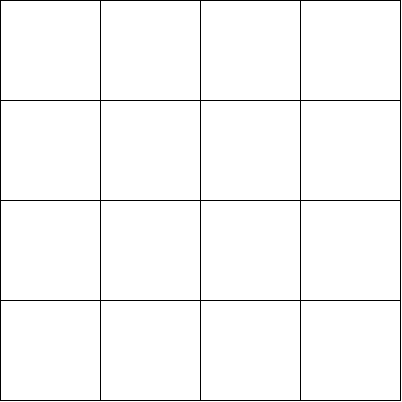
\includegraphics[scale=0.6]{nCr.png}
        \end{figure}

        \begin{sol}
            數出正方形數量,則相當於相同長度的直綫與橫綫組合:\begin{align*}
                \sum_{k=1}^{4}k^2=\frac{1}{6}(4)(4+1)(2\times 4+1)=30
            \end{align*}

            數出任意長方形數量,則相當於任意兩條直綫與任意兩條橫綫組合:\begin{align*}
                (C_2^5)^2=100
            \end{align*}

            數出純長方形數量,則相當於任意長方形的數量減去正方形的數量:\begin{align*}
                100-30=70
            \end{align*}
        \end{sol}
    \end{example}

    \begin{theorem}
        設$n,k$為正整數,$0\leq k\leq n$,則$$C_k^n=C_{n-k}^n$$
    \end{theorem}

    \begin{proof}
        \begin{align*}
            C_k^n&=\frac{n!}{k!(n-k)!}\\
            &=\frac{n!}{[n-(n-k)]!(n-k)!}\\
            &=C_{n-k}^n
        \end{align*}
    \end{proof}

    \begin{theorem}
        設$n,k$為正整數,$0\leq k< n$,則$$C_k^n+C_{k+1}^n=C_{k+1}^{n+1}$$
    \end{theorem}

    \begin{proof}
        \begin{align*}
            C_k^n+C_{k+1}^n&=\frac{n!}{k!(n-k)!}+\frac{n!}{(k+1)!(n-k-1)!}\\
            &=\frac{(k+1)n!}{(k+1)!(n-k)!}+\frac{(n-k)n!}{(k+1)!(n-k)!}\\
            &=\frac{(n+1)n!}{(k+1)!(n-k)!}\\
            &=\frac{(n+1)!}{(k+1)![(n+1)-(k+1)]!}\\
            &=C_{k+1}^{n+1}
        \end{align*}
    \end{proof}

    \section*{二項式定理}

    一般而言,面對二項式展開,會提及\textbf{帕斯卡三角}:

    \begin{figure}[H]
        \centering
        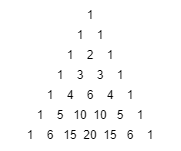
\includegraphics[scale=1]{pascal_triangle.png}
        \caption{Pascal Triangle 帕斯卡三角}
    \end{figure}

    對於二項式展開的係數,除了以帕斯卡三角為入門設想,我們亦可考慮$$\prod_{i=1}^{n}(a+b)=(a+b)^n=\sum_{i=0}^{n}ka^ib^{n-i}$$

    已知展開式中任意一項的表達式必爲$ka^xb^y$,其中$x+y=n$及$k$為常數。現求對應的$k$的值,考慮$$a^xb^y=(\prod_{i=1}^{x}a)(\prod_{j=1}^{y}b)$$

    換言之,我們需從$n$個括號中取$x$個$a$相乘,取$y$個$b$相乘,其組合數為$C_x^n C_y^{n-x}=C_x^n$。

    \begin{theorem}[二項式定理]
        設$a,b$為複數,$n$為正整數,則$$(a+b)^n=\sum_{k=0}^{n}C_k^n a^kb^{n-k}$$
    \end{theorem}

    從二項式定理延伸,可得以下多項式定理:

    \begin{definition}[多項式係數]
        定義多項式係數為$$\begin{pmatrix}
            n\\x_1,x_2,\dots,x_k
        \end{pmatrix}=\frac{n!}{x_1!x_2!\cdots x_k!}$$
    \end{definition}

    \begin{remark}
        對於二項式,若將其視爲多項式的特殊情況,則可簡記$\begin{pmatrix}
            n\\x_1,x_2
        \end{pmatrix}$為$\begin{pmatrix}
            n\\x_1
        \end{pmatrix}=C_{x_1}^n$。
    \end{remark}

    \begin{theorem}[多項式定理]
        設$a_1,a_2,\dots,a_m$為一組數,$n$為正整數,則$$(a_1+a_2+\cdots+a_m)^n=\sum_{i_1+i_2+\cdots+i_m=n}\begin{pmatrix}
            n\\i_1,i_2,\dots,i_m
        \end{pmatrix}a_1^{i_1}a_2^{i_2}\cdots a_m^{i_m}$$
    \end{theorem}

    \begin{proof}
        詳見習題11。
    \end{proof}

    \section*{習題}
    \begin{enumerate}
        \item 求$(3x^2-\frac{7}{x})^6$的常數項及$x^2$的係數。
        \item 設$(2+5x)^n-(2-3x)^n$中$x^2$的係數為10752,求$x^3$的係數。
        \item 已知$(1+kx^3)^n=1-8x^3+24x^6+\cdots$,求$k$和$n$的值,其中$n$為正整數。
        \item 已知$(1-2x)^m(1+x)^n=1-8x+18x^2+\cdots$,求$m$和$n$的值,其中$m,n$均為正整數。
        \item 求$(x+\frac{1}{x})^4(1-\frac{1}{x})^6$的常數項。
        \item 證明若$n,k$為正整數,$0\leq k< n$,則$C_k^n+C_{k+1}^n=C_{k+1}^{n+1}$。
        \item \begin{enumerate}
            \item 求$\sum_{k=0}^n C_k^n$。[HINT:考慮$(1+1)^n$的展開式。]
            \item 證明$\sum_{\textrm{奇數}k}^n C_k^n=\sum_{\textrm{偶數}k}^n C_k^n$。[HINT:考慮$(1-1)^n$的展開式。]
        \end{enumerate}
        \item 設$n$為正整數。\begin{enumerate}
            \item 設$r$為介乎1與$n$之間的正整數。證明$\frac{C_{r+1}^{n+1}}{C_r^{n+1}}=\frac{n+1-r}{r+1}$。
            \item 由此,證明一下等式:\begin{enumerate}
                \item $\displaystyle \sum_{k=0}^{n}(k+1)\cdot\frac{C_{k+1}^{n+1}}{C_k^{n+1}}=\frac{An^2+Bn+C}{2}$;
                \item $\displaystyle \prod_{k=0}^{n}(C_{k+1}^{n+1}+C_{k}^{n+1})=\frac{(n+D)^{n+E}}{[(n+F)!]}\cdot (\prod_{k=0}^{n}C_k^{n+1})$.
            \end{enumerate}
            其中$A,B,C,D,E,F$為常數,並須在結論時明確指出其值。
        \end{enumerate}
        \item 證明范德蒙定理:\begin{theorem}
            設$p,q,r$為非負整數。若$r\leq p+q$,則$\sum_{k=0}^{r}C_k^p C_{r-k}^q=C_r^{p+q}$。
        \end{theorem}
        [HINT:考慮$(1+x)^{p+q}=(1+x)^p(1+x)^q$]
        \item 求以下算式的值,並以$n$表示:\begin{enumerate}
            \item $\sum_{k=0}^{n}(C_k^n)^2$。
            \item $\sum_{k=0}^{n}(-1)^k(C_k^n)^2$
            \item $\sum_{k=0}^{n}k(C_k^n)^2$。
        \end{enumerate}
        [HINT:考慮$C_k^n=C_{n-k}^n$]
        \item 記$\begin{pmatrix}
            n\\x_1,x_2,\dots,x_k
        \end{pmatrix}=\frac{n!}{x_1!x_2!\cdots x_k!}$。\begin{enumerate}
            \item 證明對於任意正整數$n$及$k\geq 2$,若$x_1+x_2+\cdots+x_k=n$,則$$\begin{pmatrix}
                n\\x_1,x_2,\dots,x_k
            \end{pmatrix}=C_{x_1}^n C_{x_2}^{n-x_1}\cdots C_{x_{k-1}}^{n-x_1-x_2-\cdots-x_{k-2}}$$
            \item 由此,證明多項式定理。
        \end{enumerate}
        \item 已知當$-1<r<1$時,$$\frac{1}{1-r}=1+r+r^2+r^3+\cdots+r^n+\cdots=\sum_{k=0}^{\infty}r^k$$證明對於任意正整數$n$及$-1<r<1$,$$\sum_{k=0}^\infty C_k^{n+k-1}r^k=\frac{1}{(1-r)^n}$$[HINT:習題1。]
        \item 設$p$為實數且$0<p<1$。設$n$為正整數。對$k$介乎$1$與$n$之間,定義$a_k=C_k^n p^k(1-p)^{n-k}$。\begin{enumerate}
            \item 證明$\sum_{k=0}^{n}a_k=1$。
            \item 證明對於任意$k$介乎$1$與$n$之間,$0<a_k<1$。
            \item 定義$\mu=\sum_{r=0}^{n}ra_r$。證明$\mu=np$。
            \item 再定義$\sigma=\sqrt{\sum_{r=0}^n (r-\mu)^2a_r}$。\begin{enumerate}
                \item 證明$\sigma^2=\sum_{r=0}^{n}r^2a_r-\mu^2$。
                \item 證明$\sum_{r=0}^{n}r(r-1)a_r=n(n-1)p^2$,由此證明$\sigma^2=np(1-p)$。
            \end{enumerate}
        \end{enumerate}
    \end{enumerate}
\end{document}
